\documentclass[12pt,a4paper]{article}
\usepackage[utf8]{inputenc}
\usepackage{amsmath}
\usepackage{amsfonts}
\usepackage{amssymb}
\usepackage{listings}
\usepackage{url}
\usepackage[bulgarian]{babel}
\usepackage{listings}
\usepackage{enumerate}
\usepackage{hyperref}
\usepackage{relsize}
\usepackage{graphicx}


\lstset{breaklines=true} 


\author{\textit{email: kalin@fmi.uni-sofia.bg}}
\title{\textsc{Задачи за задължителна самоподготовка} \\
по \\
Структури от данни и програмиране\\
\textit{Двоични дървета 2}}



\begin{document}
\maketitle


\begin{enumerate}

	\item Да се реализира метод \texttt{vector<T> BTree<T>::listLeaves ()} намиращ списък със стойностите на листата на дървото.

	\item Да се дефинира метод \texttt{string BTree<T>::findTrace (const T\& x)}. Ако \texttt{x} е елемент на дървото, функцията да връща следата на \texttt{x} (според дефиницията на ``следа'', обсъдена на лекции). Ако \texttt{x} не е елемент на дървото, функцията да връща низа ``\_''.

	\textit{Пример: За дървото от фигура 1, следата на елемента със стойност 25 е ``RR''}.

	\begin{flushleft}
	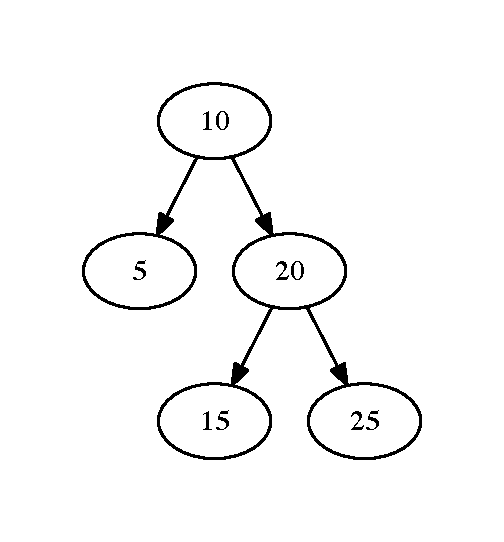
\includegraphics[width=4cm]{images/tree1}

	\relscale{0.8}
	Фигура 1. Двоично наредено дърво
	\end{flushleft}

	\item Да се дефинира метод \texttt{void BTree<T>::prettyPrint ()}, отпечатващ дървото на конзолата по следния начин: (1) всеки наследник е вдясно от родителя си, (2) елементите на еднакво ниво в дървото се отпечатват на еднаква колона от екрана, (3) десните наследници са на предишен ред от родителя си и (4) левите наследни са следващ ред спрямо родителя си.

	Например, дървото от Фигура 1 би изглеждало по следния начин (включени са номерата на редовете на конзолата):

\begin{verbatim}
1:        25
2:    20	
3:        15
4: 15
5:    5
\end{verbatim}


	\item Нека е даден израз, построен по правилата на следната грматика:

\begin{verbatim}
<expression> ::= <digit> | (<expression><operator><expresson>)
<digit> ::= 1..9
<operator> ::= + | - | * | /
\end{verbatim}

	Да се реалзира метод \texttt{void BTree<char>::parseExpression (string s)}, който по правилно построен израз, записан в низа \texttt{s}, създава двоично дърво от символи, представящо израза по следното правило:
	\begin{itemize}
		\item Ако изразът е от типа ``\texttt{x}'', където \texttt{x} е цифра, то съответното му дърво е листо със стойност символа \texttt{x}.
		\item Ако изразът е от типа ``\texttt{(<израз 1><op><израз 2>)}'', то съответното му дърво има като стойност на корена символа на съответния оператор, ляво поддърво, съответно на \texttt{<израз 1>} и дясно поддърво, съответно на \texttt{<израз 2>}.
	\end{itemize}
	
	\begin{flushleft}
	\vspace{-50px}
	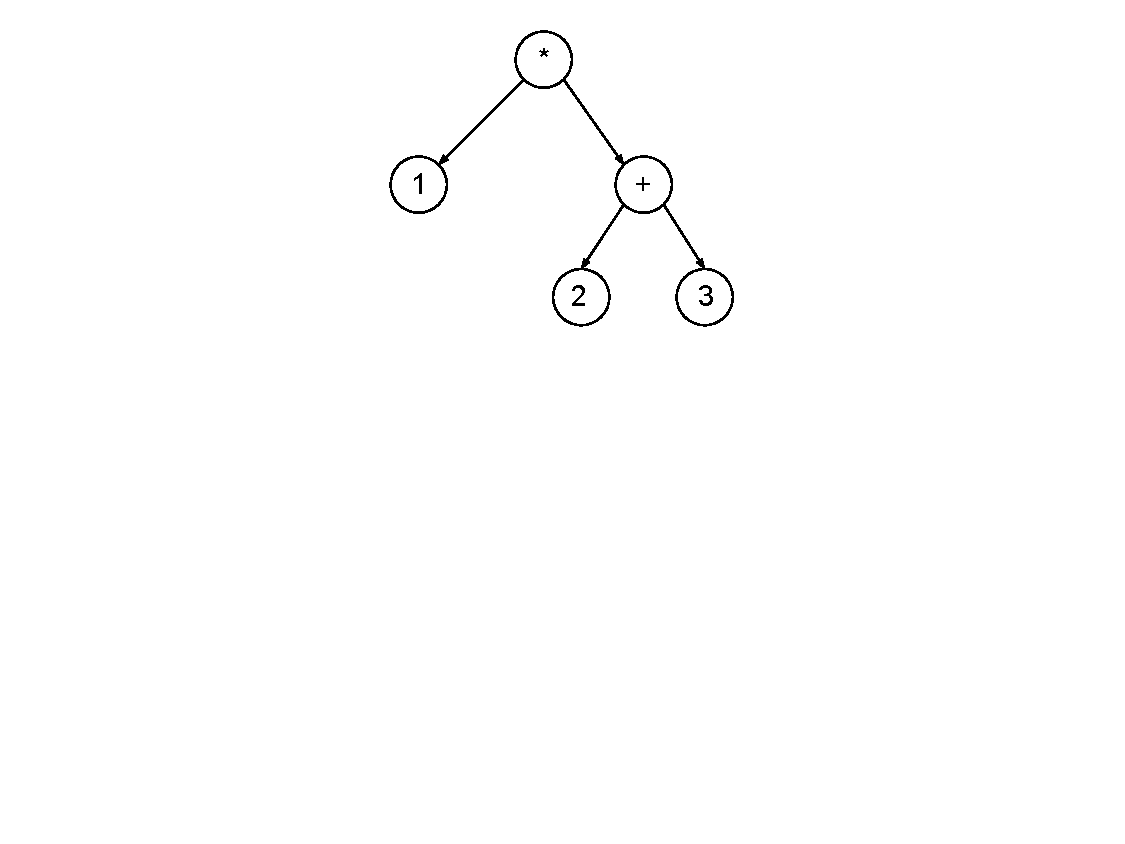
\includegraphics[width=12cm]{images/tree2}
	\vspace{-160px}

	\relscale{0.8}
	Фигура 2. Дърво на израза \texttt{(1*(2+3))}.
	\end{flushleft}

	Дървото на фигура 2 съответства на изарза \texttt{(1*(2+3))}.

	\item Да се реализира метод \texttt{double BTree<char>::calculateExpresisonTree ()}, който намира стойността на израз, построен от решението на предишната задача.

	\item Да се дефинира оператор \texttt{T\& BTree<T>::operator[](int i)}, който намира $i$-тият пореден елемент на дървото при обхождане корен-ляво-дясно. 

	Пример: За дървото от фигура 1, елементът с пореден номер 0 е 15, с номер 1 е 5, с номер 2 е 20 и т.н.

	\item Да се дефинира метод \texttt{vector<T> BTree<T>::level (int k)}, който намира и връща вектор, съдържащ стойностите на всички елементи на дървото, които са на ниво k (т.е. има път от корена до тях с дължина в брой върхове k).









\end{enumerate}






\end{document}

